\section{类 Date 的属性}
\hfill\ctli{实验时间}{~2015~年~1~月~9~日}
\subsection*{【实验目的】}
\begin{enumerate}[topsep=0pt,partopsep=0pt,itemsep=0pt,parsep=0pt,label={\arabic*、}]
\item 掌握重载的概念
\item 能够进行运算符重载。
\end{enumerate}
\subsection*{【实验环境】}
\MyEnvironment
\subsection*{【实验内容】}
日期类设计

定义Date类,参照实现:
\begin{enumerate}[topsep=0pt,partopsep=0pt,itemsep=0pt,parsep=0pt,label={(\arabic*)}]
\item 日期的加、减运算
\item 根据日期计算一年中的第几周星期几、一年中第几天为几月几日、该年是否为闰年
\item 输出日期对象
\end{enumerate}

完成相应应用程序设计
\subsection*{【详细分析】}
(此项由学生自己完成)
\subsubsection*{【实验源码】}
{\linespread{1}\lstinputlisting[caption={\tt Date.h}]{exp05/Date.h}}
{\linespread{1}\lstinputlisting[caption={\tt Date.cpp}]{exp05/Date.cpp}}
{\linespread{1}\lstinputlisting[caption={\tt exp01.cpp}]{exp05/exp01.cpp}}
\subsubsection*{【实验结果】}
\begin{figure}[htp]
\centering
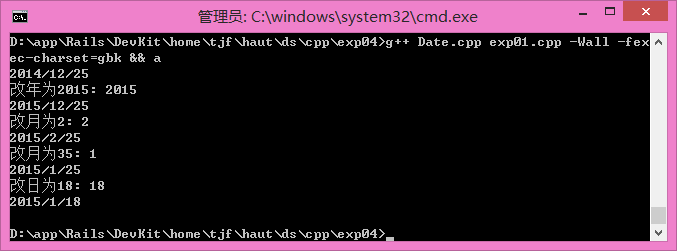
\includegraphics[width=\textwidth]{exp05/exp01.png}
\caption{\label{out05_01}Date 类}
\end{figure}
\subsection*{【实验体会】}
(至少150字)
